\documentclass[UTF8, a4paper, 11pt]{article}
\usepackage{diagbox}
\usepackage{subfigure}
\usepackage[UTF8, scheme=plain]{ctex}
\usepackage{fontspec}
\usepackage{float}
\usepackage{amsmath}
\newtheorem{myDef}{Definition}
\usepackage{graphicx}
\usepackage{geometry}
\usepackage{listings}
\usepackage{xcolor}
\usepackage{caption}
\geometry{scale=0.8}
\linespread{1.5}
\usepackage{hyperref}
\usepackage{color}
\usepackage{fontspec}
\usepackage{enumitem}
\usepackage[linesnumbered,boxed]{algorithm2e}    
\usepackage{xeCJK}
\usepackage{indentfirst} 
\usepackage{amssymb}
\graphicspath{{Pics/}} 	% 在于.tex同级的目录下创建名为pic的文件夹,存放图片


\setlength{\parindent}{2em}

\lstset{
    language={python},
    frame=shadowbox,
    breaklines=true,
    numbers=left,
    backgroundcolor=\color[RGB]{245,245,244},
    rulesepcolor=\color{red!20!green!20!blue!20},
    numberstyle={\color[RGB]{0,192,192}\tiny},
    basicstyle=\footnotesize \fontspec{Source Code Pro}
}
\setenumerate[1]{itemsep=0pt,partopsep=0pt,parsep=\parskip,topsep=0pt}
\setitemize[1]{itemsep=0pt,partopsep=0pt,parsep=\parskip,topsep=0pt}
\setdescription{itemsep=0pt,partopsep=0pt,parsep=\parskip,topsep=0pt}


\title{	
\normalfont \normalsize
\textsc{School of Data and Computer Science, Sun Yat-sen University} \\ [25pt] %textsc small capital letters
\rule{\textwidth}{0.5pt} \\[0.4cm] % Thin top horizontal rule
\huge 数电实验11\\ % The assignment title
\rule{\textwidth}{2pt} \\[0.5cm] % Thick bottom horizontal rule
\author{18308045 谷正阳}
\date{\normalsize\today}
}

\begin{document}
\maketitle
\tableofcontents
\newpage
\section{仿真实验}
\subsection{显示学号}
\subsubsection{电路图}
\begin{figure}[H]
    \centering
    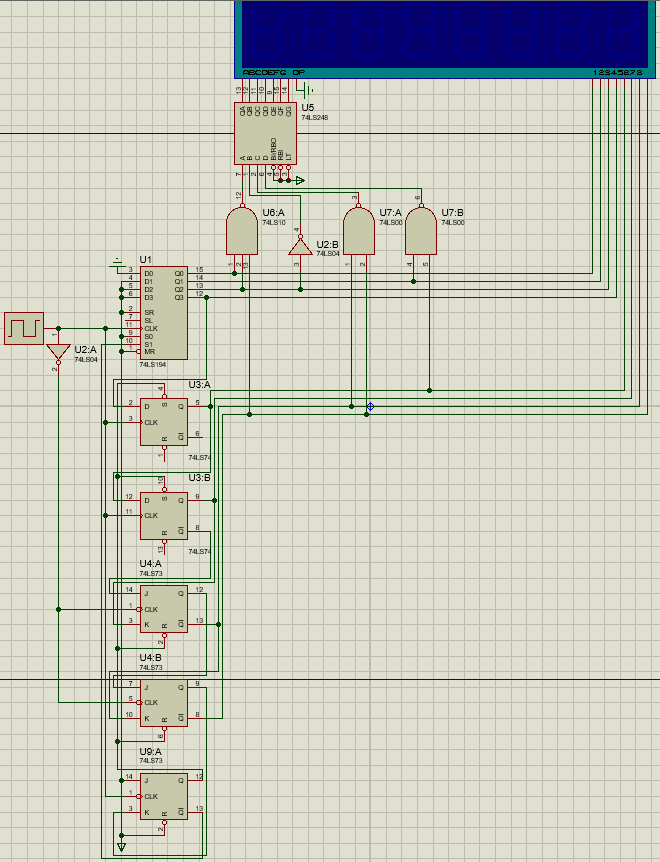
\includegraphics[width=0.8\textwidth]{ex11.1电路图.png}
\end{figure}
用2个D触发器,2个JK触发器实现1个4位移位寄存器。
再用1个现成的移位寄存器构成8位移位寄存器。
8位移位寄存器初始化为01111111,最后用一个JK触发器,判断到最右端输出0时置初值,实现ring counter,且无需手动置初值。

4位移位寄存器和D触发器都有置位和清零可以直接置需要的初值。
JK触发器只有清零端,但是若把$\overline Q$视作$Q$,即可认为清零是置位,此时还需把$J$视作$K$,把$K$视作$J$。

Ring counter扫描LED的位置码,不同位置码使用组合逻辑电路产生所需BCD码,真值表如下:
\begin{table}[H]
    \center
\begin{tabular}{|l|l|l|l|l|l|l|l|l|l|l|l|l|}
\hline
$Q_0$ & $Q_1$ & $Q_2$ & $Q_3$ & $Q_4$ & $Q_5$ & $Q_6$ & $Q_7$ & $N$ & $A$ & $B$ & $C$ & $D$ \\ \hline
0  & 1  & 1  & 1  & 1  & 1  & 1  & 1  & 1 & 1 & 0 & 0 & 0 \\ \hline
1  & 0  & 1  & 1  & 1  & 1  & 1  & 1  & 8 & 0 & 0 & 0 & 1 \\ \hline
1  & 1  & 0  & 1  & 1  & 1  & 1  & 1  & 3 & 1 & 1 & 0 & 0 \\ \hline
1  & 1  & 1  & 0  & 1  & 1  & 1  & 1  & 0 & 0 & 0 & 0 & 0 \\ \hline
1  & 1  & 1  & 1  & 0  & 1  & 1  & 1  & 8 & 0 & 0 & 0 & 1 \\ \hline
1  & 1  & 1  & 1  & 1  & 0  & 1  & 1  & 0 & 0 & 0 & 0 & 0 \\ \hline
1  & 1  & 1  & 1  & 1  & 1  & 0  & 1  & 4 & 0 & 0 & 1 & 0 \\ \hline
1  & 1  & 1  & 1  & 1  & 1  & 1  & 0  & 5 & 1 & 0 & 1 & 0 \\ \hline
\end{tabular}
\end{table}
在某几个$Q$为0时,输出1,否则输出0,是与非的关系。
\subsubsection{结果}
\begin{figure}[H]
    \centering
    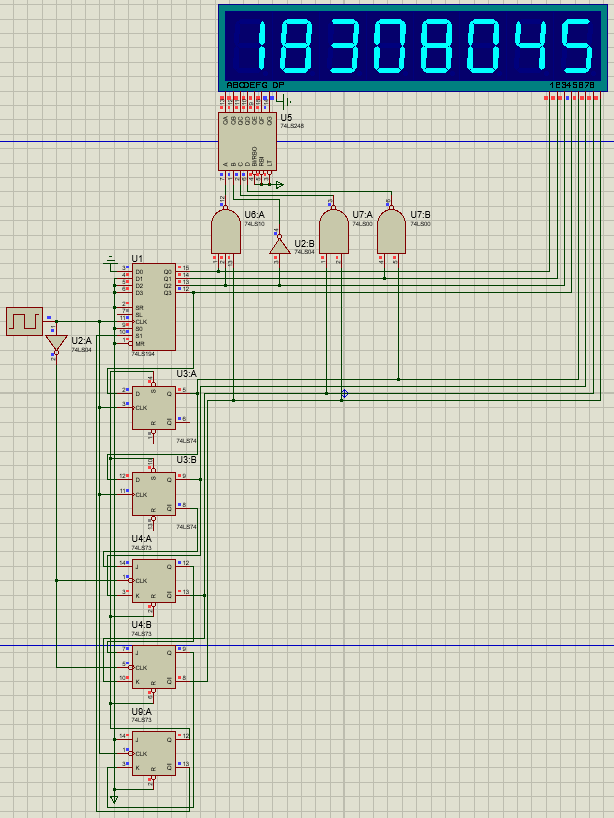
\includegraphics[width=0.8\textwidth]{ex11.1结果.png}
\end{figure}
\subsection{学号双向计数器}
\subsubsection{电路图}
\begin{figure}[H]
    \centering
    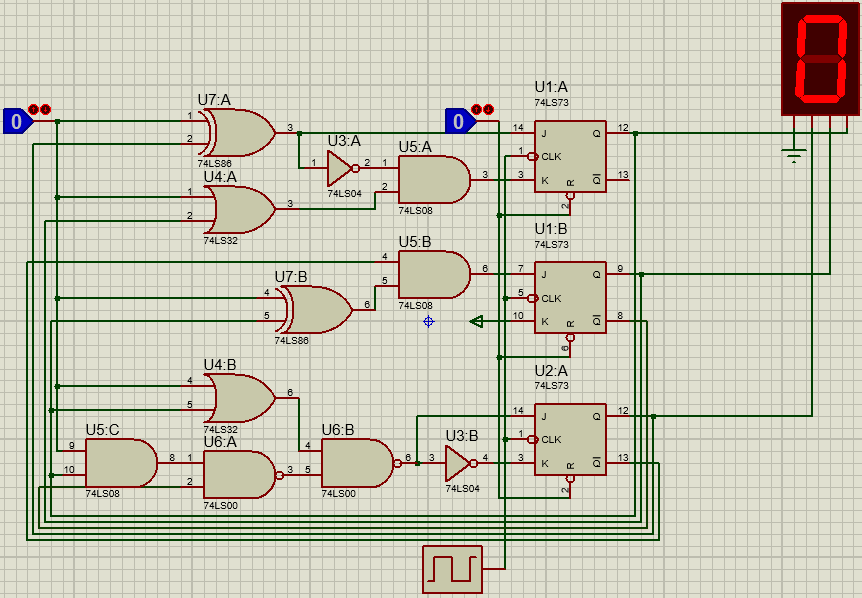
\includegraphics[width=0.8\textwidth]{ex11.2电路图.png}
\end{figure}
右边使能端高电平有效,左边控制端低电平正向计数13045,高电平反向计数54021。
\begin{table}[H]
    \center
\begin{tabular}{|l|l|l|l|l|l|l|l|l|}
\hline
$Q(t)$ & $Q(t+1)$ & $Q(t)_2$ & $Q(t)_1$ & $Q(t)_0$ & $Q(t+1)_2$ & $Q(t+1)_1$ & $Q(t+1)_0$ & $S$ \\ \hline
1      & 3        & 0        & 0        & 1        & 0          & 1          & 1          & 0   \\ \hline
3      & 0        & 0        & 1        & 1        & 0          & 0          & 0          & 0   \\ \hline
0      & 4        & 0        & 0        & 0        & 1          & 0          & 0          & 0   \\ \hline
4      & 5        & 1        & 0        & 0        & 1          & 0          & 1          & 0   \\ \hline
5      & 1        & 1        & 0        & 1        & 0          & 0          & 1          & 0   \\ \hline
5      & 4        & 1        & 0        & 1        & 1          & 0          & 0          & 1   \\ \hline
4      & 0        & 1        & 0        & 0        & 0          & 0          & 0          & 1   \\ \hline
0      & 3        & 0        & 0        & 0        & 0          & 1          & 1          & 1   \\ \hline
3      & 1        & 0        & 1        & 1        & 0          & 0          & 1          & 1   \\ \hline
1      & 5        & 0        & 0        & 1        & 1          & 0          & 1          & 1   \\ \hline
\end{tabular}
\end{table}

绘制$Q(t+1)_0$卡诺图
\begin{table}[H]
    \center
\begin{tabular}{|l|l|l|l|l|}
\hline
\diagbox{$Q_2Q_1$}{$Q_0S$} & 00 & 01 & 11 & 10 \\ \hline
00                         & 0  & 1  & 1  & 1  \\ \hline
01                         & X  & X  & 1  & 0  \\ \hline
11                         & X  & X  & X  & X  \\ \hline
10                         & 1  & 0  & 0  & 1  \\ \hline
\end{tabular}
\end{table}
$$
\begin{aligned}
    \because
    &\begin{cases}
        &Q(t+1)_0\\
        =&Q(t)_2\cdot S'+Q(t)_2'\cdot S+Q(t)_1'\cdot Q(t)_0\cdot S'\\
        =&Q(t)_2\oplus S\cdot(Q(t)_0'+Q(t)_0)+Q(t)_1'\cdot Q(t)_0\cdot S'\\
        =&(Q(t)_2\oplus S)\cdot Q(t)_0'+(Q(t)_2\oplus S+Q(t)_1'\cdot S')\cdot Q(t)_0\\
        &Q(t+1)_0\\
        =&J_0\cdot Q(t)_0'+K_0'\cdot Q(t)_0
    \end{cases}\\
    \therefore
    &\begin{cases}
        &J_0\\
        =&Q(t)_2\oplus S\\
        &K_0'\\
        =&Q(t)_2\oplus S+Q(t)_1'\cdot S'\\
        =&J_0+Q(t)_1'\cdot S'\\
        =&(J_0'\cdot(Q(t)_1+S))'
    \end{cases}\\
    \therefore
    &\begin{cases}
        J_0=&Q(t)_2\oplus S\\
        K_0=&J_0'\cdot(Q(t)_1+S)
    \end{cases}
\end{aligned}
$$
$J_0$可以复用。

绘制$Q(t+1)_1$卡诺图
\begin{table}[H]
    \center
\begin{tabular}{|l|l|l|l|l|}
\hline
\diagbox{$Q_2Q_1$}{$Q_0S$} & 00 & 01 & 11 & 10 \\ \hline
00                         & 0  & 1  & 0  & 1  \\ \hline
01                         & X  & X  & 0  & 0  \\ \hline
11                         & X  & X  & X  & X  \\ \hline
10                         & 0  & 0  & 0  & 0  \\ \hline
\end{tabular}
\end{table}
$$
\begin{aligned}
    \because
    &\begin{cases}
        &Q(t+1)_1\\
        =&Q(t)_2'\cdot Q(t)_0'\cdot S+Q(t)_2'\cdot Q(t)_1'\cdot Q(t)_0\cdot S'\\
        =&Q(t)_2'\cdot Q(t)_0'\cdot S\cdot (Q(t)_1'+Q(t)_1)+Q(t)_2'\cdot Q(t)_1'\cdot Q(t)_0\cdot S'\\
        =&(Q(t)_2'\cdot Q(t)_0'\cdot S+Q(t)_2'\cdot Q(t)_0\cdot S')\cdot Q(t)_1'+Q(t)_2'\cdot Q(t)_0'\cdot S\cdot Q(t)_1\\
        &Q(t+1)_1\\
        =&J_1\cdot Q(t)_1'+K_1'\cdot Q(t)_1
    \end{cases}\\
    \therefore
    &\begin{cases}
        &J_1\\
        =&Q(t)_2'\cdot Q(t)_0'\cdot S+Q(t)_2'\cdot Q(t)_0\cdot S'\\
        =&Q(t)_2'\cdot (Q(t)_0\oplus S)\\
        &K_1'\\
        =&Q(t)_2'\cdot Q(t)_0'\cdot S\\
        =&0(\because Q2,Q0不同时为0
    \end{cases}\\
    \therefore
    &\begin{cases}
        J_1=&Q(t)_2'\cdot (Q(t)_0\oplus S)\\
        K_1=&1
    \end{cases}
\end{aligned}
$$

绘制$Q(t+1)_2$卡诺图
\begin{table}[H]
    \center
\begin{tabular}{|l|l|l|l|l|}
\hline
\diagbox{$Q_2Q_1$}{$Q_0S$} & 00 & 01 & 11 & 10 \\ \hline
00                         & 1  & 0  & 1  & 0  \\ \hline
01                         & X  & X  & 0  & 0  \\ \hline
11                         & X  & X  & X  & X  \\ \hline
10                         & 1  & 0  & 1  & 0  \\ \hline
\end{tabular}
\end{table}
$$
\begin{aligned}
    \because
    &\begin{cases}
        &Q(t)_0'\cdot S'+Q(t)_1'\cdot Qt(0)\cdot S\\
        =&(Q(t)_0'\cdot S'+Q(t)_1'\cdot Qt(0)\cdot S)\cdot(Q(t)_2'+Q(t)_2)\\
        =&(Q(t)_0'\cdot S'+Q(t)_1'\cdot Qt(0)\cdot S)\cdot Q(t)_2'+(Q(t)_0'\cdot S'+Q(t)_1'\cdot Qt(0)\cdot S)\cdot Q(t)_2\\
        &Q(t+1)_2\\
        =&J_2\cdot Q(t)_2'+K_2'\cdot Q(t)_2
    \end{cases}\\
    \therefore
    &\begin{cases}
        &J_2\\
        =&Q(t)_0'\cdot S'+Q(t)_1'\cdot Qt(0)\cdot S\\
        =&((Q(t)_0'\cdot S')'\cdot(Q(t)_1'\cdot Qt(0)\cdot S)')'\\
        =&((Q(t)_0+S)\cdot (Q(t)_1'\cdot Qt(0)\cdot S)')'\\
        &K_2'\\
        =&Q(t)_0'\cdot S'+Q(t)_1'\cdot Qt(0)\cdot S\\
        =&J_2\\
    \end{cases}\\
    \therefore
    &\begin{cases}
        J_2=&((Q(t)_0+S)\cdot(Q(t)_1'\cdot Qt(0)\cdot S)')'\\
        K_2=&J_2'
    \end{cases}
\end{aligned}
$$
$J_2$可以复用。
\subsubsection{结果}
\href{run:./1.mp4}{点击查看演示视频1.mp4}
\section{实验箱实验}
\subsection{显示学号}
\begin{figure}[H]
    \centering
    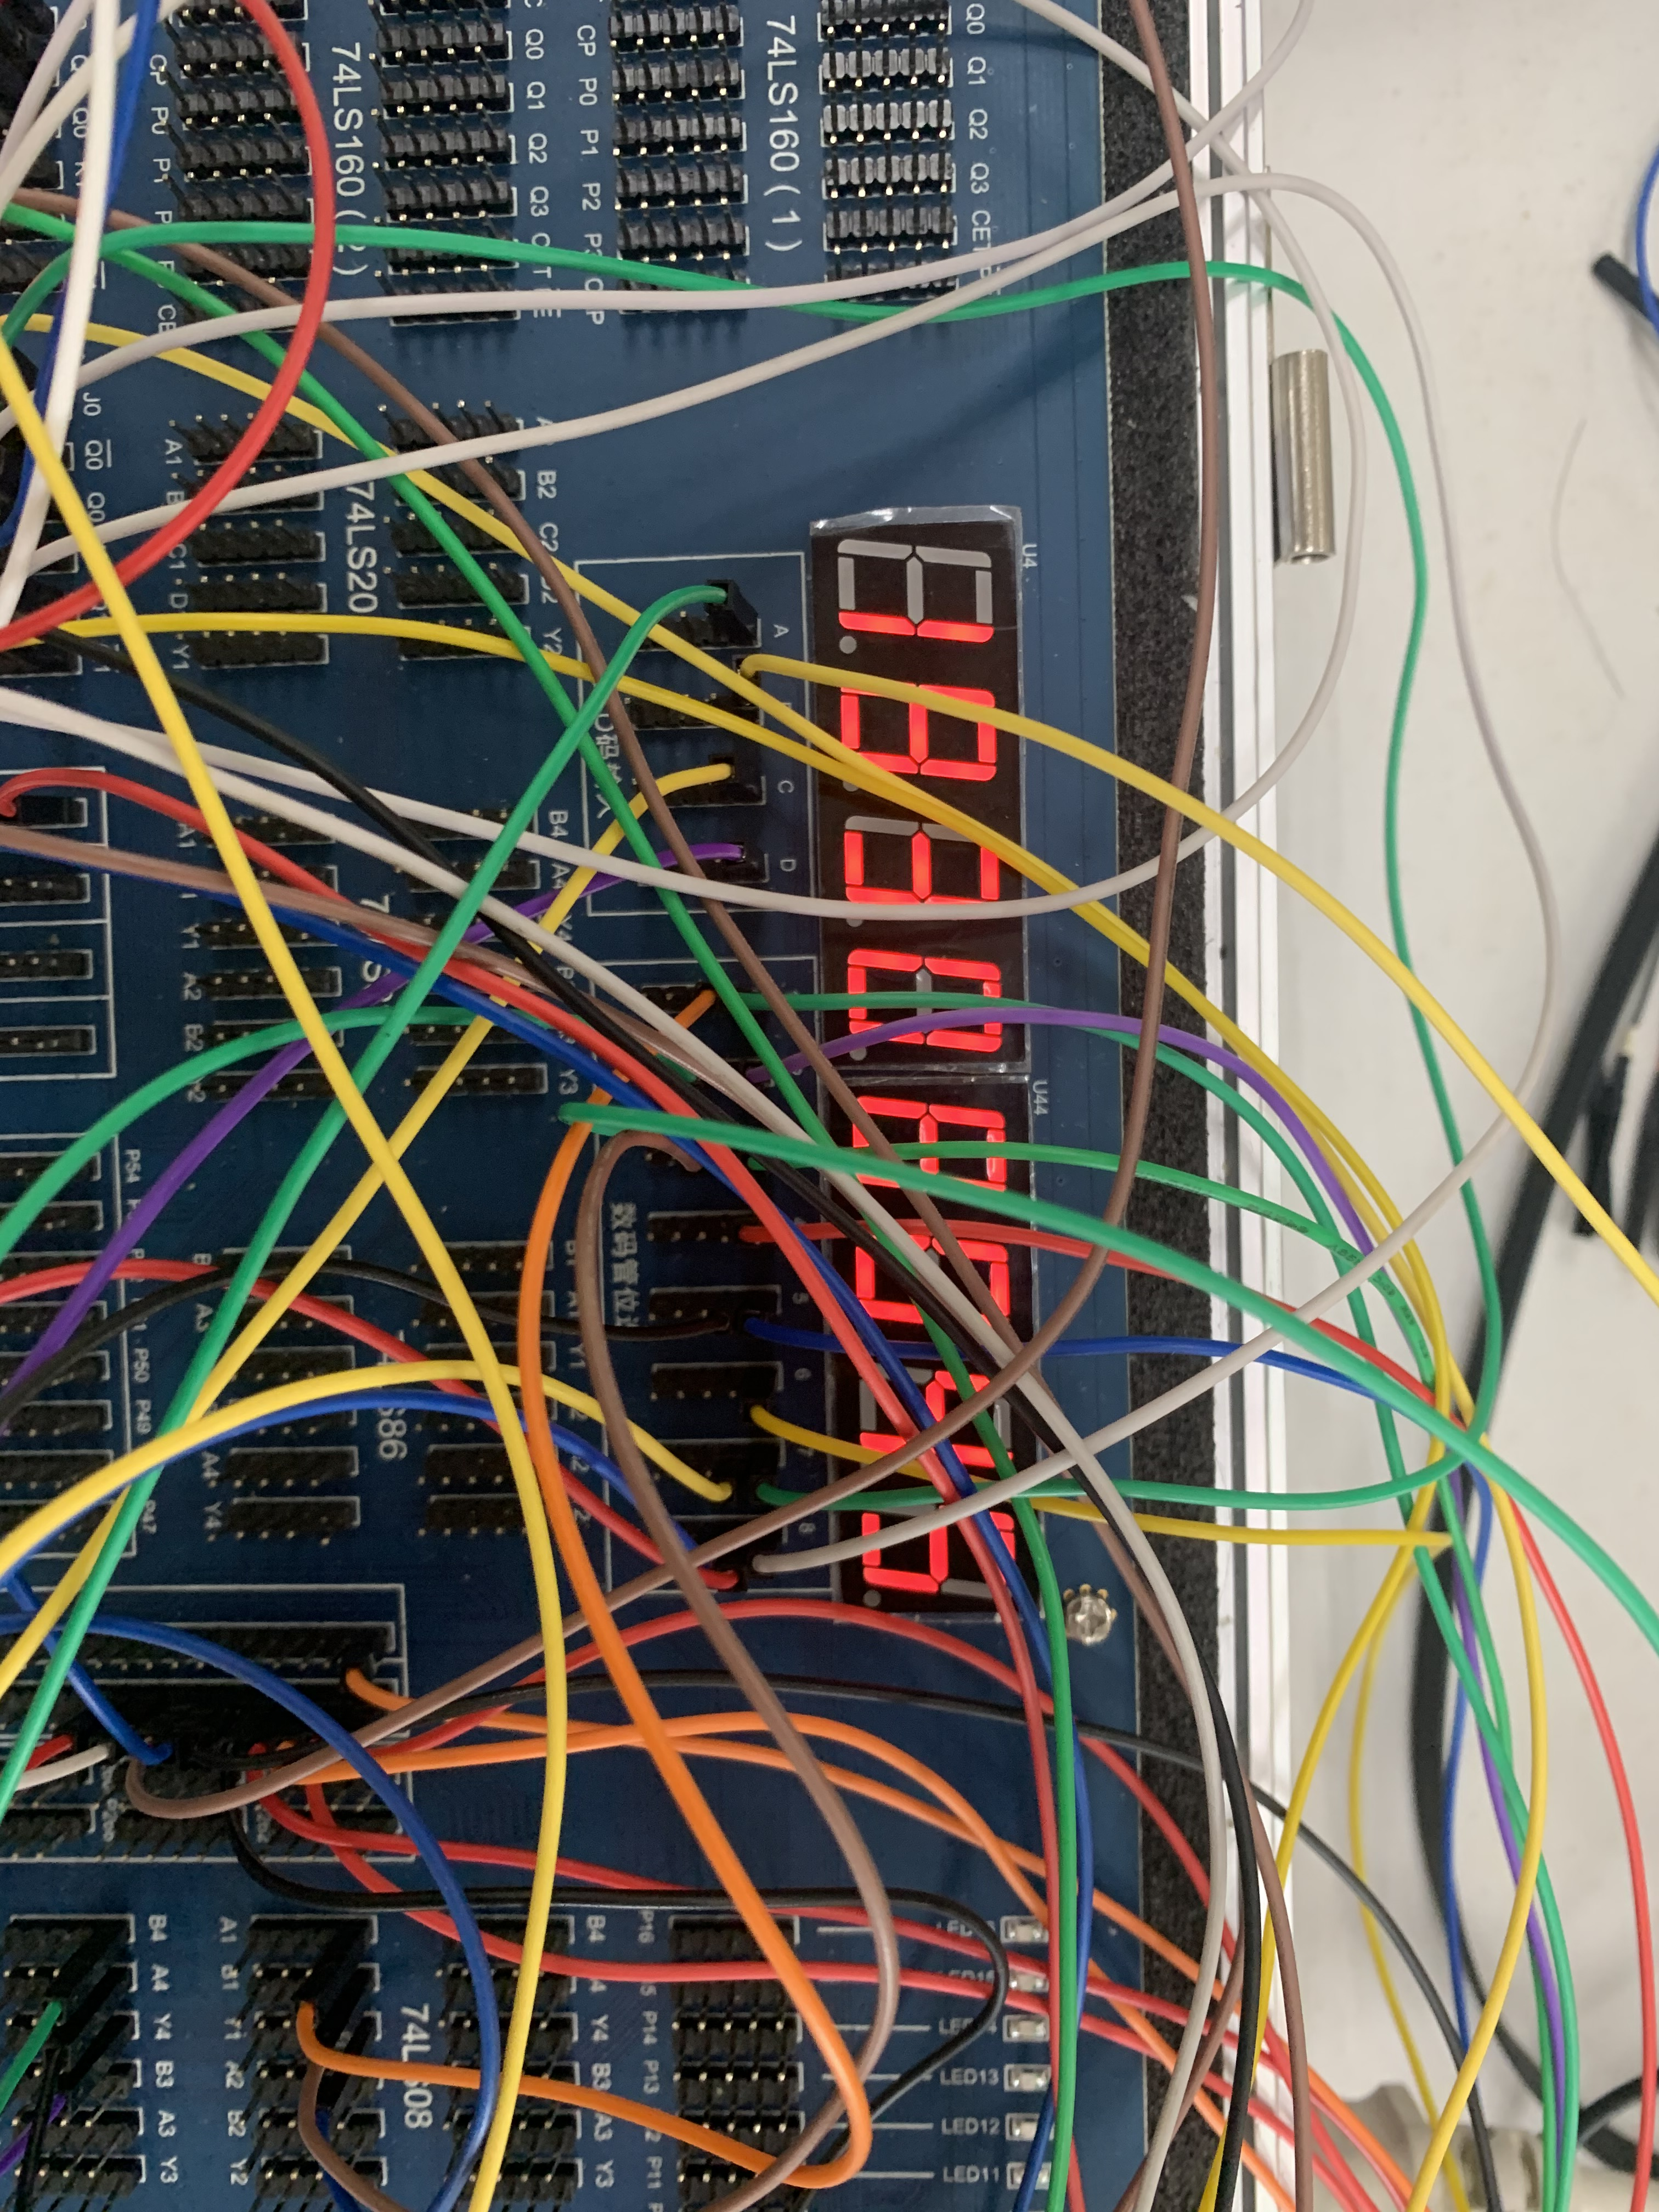
\includegraphics[width=0.8\textwidth]{学号.jpg}
\end{figure}
%\clearpage
%\bibliography{E:/Papers/LiuLab}
%\bibliographystyle{apalike}
\end{document}
%%% Local Variables:
%%% mode: latex
%%% TeX-master: t
%%% End:
